% !TEX root = ../../../main.tex
% 来源：中学数学实验教材·第三册（高中数学）
% 章节：不等式和解不等式 / 解不等式
% 原始文件：3.tex，行 2118-2150
% 类型：tikz
% ---
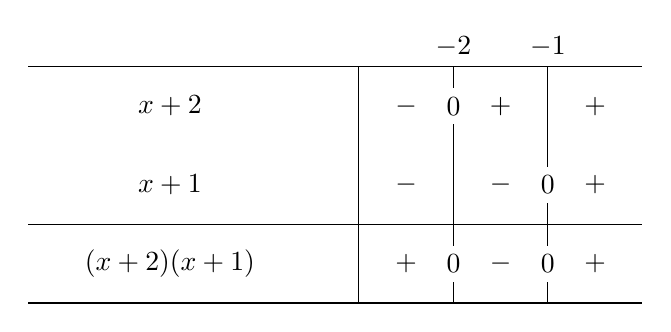
\begin{tikzpicture}[yscale=2, xscale=1.2]
\foreach \x in {0,.5,1.5}
{
    \draw (2,\x)--(8.5,\x);
}
\foreach \x/\xtext in {5.5/{},6.5/-2,7.5/-1}
{
    \draw (\x,0)--(\x,1.5)node[above]{$\xtext$};
}

\node at (3.5,.25){$(x+2)(x+1)$};
\foreach \x/\xtext in {6/+,7/-,8/+}
{
    \node at (\x,.25) {$\xtext$};
}

\node at (3.5,.75){$x+1$};
\foreach \x/\xtext in {6/-,7/-,8/+}
{
    \node at (\x,.75) {$\xtext$};
}

\node at (3.5,1.25){$x+2$};
\foreach \x/\xtext in {6/-,7/+,8/+}
{
    \node at (\x,1.25) {$\xtext$};
}

\node at (6.5,.25)[fill=white] {0};
\node at (7.5,.25)[fill=white] {0};
\node at (7.5,.75)[fill=white] {0};
\node at (6.5,1.25)[fill=white] {0};
\end{tikzpicture}
